% !TEX encoding = UTF-8 Unicode

\documentclass[11pt,a4paper]{article}

\usepackage[T1]{fontenc}
\usepackage[utf8]{inputenc}

\usepackage[sc]{mathpazo}
\linespread{1.05} % Line spacing - Palatino needs more space between lines
\usepackage{microtype} % Slightly tweak font spacing for aesthetics

\usepackage{geometry}
\usepackage[pdftex]{graphicx}

\usepackage{amsmath}
\usepackage{amssymb}
\usepackage{amsthm}

\usepackage{epstopdf}

\usepackage[font=footnotesize,labelfont=bf]{caption}
\usepackage[font=footnotesize,labelfont=bf]{subcaption}
\usepackage{hyphenat}
\usepackage[inline]{enumitem}

\usepackage{xcolor}
\usepackage{mathrsfs}
\newtheorem{theorem}{Theorem}
\newtheorem{corollary}{Corollary}
\newtheorem{prop}{Proposition}
\theoremstyle{definition}
\newtheorem{example}{Example}
\newtheorem{definition}{Definition}

% vast and Vast brackets (larger than Huge)
\makeatletter
\newcommand{\HUGE}{\bBigg@{3}}
\newcommand{\vast}{\bBigg@{4}}
\newcommand{\Vast}{\bBigg@{5}}
\makeatother
% Math in header should be boldface
\makeatletter
\g@addto@macro\bfseries{\boldmath}
\makeatother

% My own commands
\usepackage{gensymb} % degree sign
\renewcommand{\epsilon}{\varepsilon}
\renewcommand{\phi}{\varphi}

\newcommand{\fr}[2]{\frac{#1}{#2}}
\newcommand{\pf}[2]{\dfrac{\partial #1}{\partial #2}}
\newcommand{\cd}{\cdot}
% \newcommand{\T}{\!\mathsf{T}}
\newcommand{\T}{T}
\newcommand{\te}[1]{\text{#1}}
\newcommand{\id}{\mathrm{d}}
\usepackage{bm}
\newcommand{\mat}[1]{\bm{#1}}
\newcommand{\nullspace}[1]{\mathcal{N}{#1}}
\newcommand{\lagrange}[1]{\mathcal{L}{#1}}
\usepackage{mathtools}

\usepackage{bbm}
\newcommand{\N}{\ensuremath{\mathbbm{N}}}
\newcommand{\Z}{\ensuremath{\mathbbm{Z}}}
\newcommand{\Q}{\ensuremath{\mathbbm{Q}}}
\newcommand{\R}{\ensuremath{\mathbbm{R}}}
\newcommand{\K}{\ensuremath{\mathbbm{K}}}
\newcommand{\C}{\ensuremath{\mathbbm{C}}}

\newcommand{\lr}{\ensuremath{\mathrm{\quad\Leftrightarrow\quad}}}
\newcommand{\ra}{\ensuremath{\mathrm{\quad\Rightarrow\quad}}}
\newcommand{\lra}{\ensuremath{\mathrm{\longrightarrow}}}
\newcommand{\f}[3]{#1\,:\,#2\,\lra\,#3}
\newcommand{\norm}[1]{\left\|#1\right\|}
\DeclareMathOperator{\sgn}{sgn}
\DeclareMathOperator{\syz}{Syz}
\DeclareMathOperator{\diag}{diag}
\DeclareMathOperator{\atan}{atan2}
\DeclareMathOperator{\tr}{tr}
\DeclareMathOperator{\adj}{adj}
\DeclareMathOperator*{\argmax}{argmax}
\DeclareMathOperator{\nulldim}{nulldim}
\DeclareMathOperator{\rank}{rank}
\DeclareMathOperator{\lt}{LT}
\DeclareMathOperator{\sat}{Sat}
\newcommand{\Rop}[1]{\mathcal{R}_{#1}}

\makeatletter
\DeclareRobustCommand\eg{\emph{e.g}\@ifnextchar.{}{.\@}}
\DeclareRobustCommand\etal{\emph{et~al}\@ifnextchar.{}{.\@}}
\DeclareRobustCommand\ie{\emph{i.e}\@ifnextchar.{}{.\@}}
\DeclareRobustCommand\cf{\emph{cf}\@ifnextchar.{}{.\@}}
\DeclareRobustCommand\NB{\emph{N.B}\@ifnextchar.{}{.\@}}
\DeclareRobustCommand\wrt{w.r.t\@ifnextchar.{}{.\@}}
\makeatother

\newcommand{\CE}{\ensuremath{\mat{C}_\mathcal{E}}}
\newcommand{\CR}{\ensuremath{\mat{C}_\mathcal{R}}}
\newcommand{\CB}{\ensuremath{\mat{C}_\mathcal{B}}}
\newcommand{\CEk}[1]{\ensuremath{\mat{C}_{\mathcal{E}_{#1}}}}
\newcommand{\CRk}[1]{\ensuremath{\mat{C}_{\mathcal{R}_{#1}}}}
\newcommand{\CBk}[1]{\ensuremath{\mat{C}_{\mathcal{B}_{#1}}}}
\newcommand{\XE}{\ensuremath{\mat{X}_\mathcal{E}}}
\newcommand{\XR}{\ensuremath{\mat{X}_\mathcal{R}}}
\newcommand{\XB}{\ensuremath{\mat{X}_\mathcal{B}}}

\graphicspath{{./images/}}

\usepackage{hyperref}
\usepackage[capitalise,noabbrev]{cleveref}

% Use paragraph for "Practical examples"
\usepackage{titlesec}
\titleformat*{\paragraph}{\itshape\mdseries}
\newcommand{\pexamples}{\paragraph{Practical examples:}}

% Fix apalike
\usepackage[square]{natbib}

%----------------------------------------------------------------------------------------
%   TITLE SECTION
%----------------------------------------------------------------------------------------

\title{
\normalfont \normalsize
\textsc{Lund University --- Algebraic Geometry} \\ [7pt]
\Large Practical aspects of solving a system of polynomial equations \\
}
\author{Marcus Valtonen \"{O}rnhag} % Your name

\date{\normalsize\today} % Today's date or a custom date

\begin{document}

\maketitle % Print the title

\section{Introduction}
In this lecture, we will discuss how to optimize the computations, both for speed and
accuracy, given a polynomial system of equations with generic coefficients. Such problems are very
frequent in computer vision, and many of the examples will be from this field of research.
I will mostly rely on examples; however,
the necessary theory is briefly discussed in this document, which you are encouraged to read before
the lecture. The theory is not meant to be complete, and I will refer you to other sources for
each topic, and try to list actual publications using the particular method.

For the practical part, we will use the
automatic solver by Larsson~\etal{}, which you should install and get accustomed to prior
to the lecture. The solver is available at~\url{http://people.inf.ethz.ch/vlarsson/misc/autogen_v0_5.zip} and requires Macaulay2 to be installed. If you want to use C++ (which greatly decreases the computation time) you will need to install the Eigen library as well.\footnote{There is also a wrapped version by Bo Li~\url{https://github.com/prclibo/gaps}, that you might prefer.}
Apart from the course literature, you are also referred to Viktor Larsson's PhD
thesis for a deeper understanding of the content in this lecture~\cite{larsson-phd}.
Examples marked with (*) have a code snippet associated with them and will be discussed during the
lecture in more detail.

\section{Theory}
\subsection{Recapitulation of the course contents}
Using multi-index notation,
let~$\mat{x^{\alpha}}$ denote a \emph{monomial} of degree $|\mat{\alpha}|$.
Our main goal is to solve a polynomial system of equations
\begin{equation}\label{kappa:eq:polsys}
    \begin{aligned}
    f_1(\mat{x}) & = 0, \\
                 & \hspace{0.575em} \vdots \\
    f_s(\mat{x}) & = 0,
    \end{aligned}
\end{equation}
where each polynomial equation can be expressed
as~$f=\sum_{\mat{\alpha}}c_{\mat{\alpha}}\mat{x^\alpha}$.
The set of all solutions to~\eqref{kappa:eq:polsys} is called an \emph{affine variety}, and is denoted
$\mat{V}(f_1,\ldots,f_s)\subset\C$.
Let~$\C[\mat{x}]$ denote the set
of polynomials in~$\mat{x}$ with coefficients in $\C$.
An \emph{ideal} $I\subset\C[\mat{x}]$ is an additive group satisfying the \emph{absorption property},~\ie{}~if~$f\in I$
and $h\in\C[\mat{x}]$ then $hf\in I$. Moreover, given a set of polynomials $f_1,\ldots,f_s\in\C[\mat{x}]$
we consider the ideal
\begin{equation}
\langle f_1,\ldots,f_s\rangle = \left\{\sum_{i=1}^sh_if_i\;:\;h_1,\ldots,h_s\in\C[\mat{x}]\right\},
\end{equation}
which we will refer to as the \emph{ideal generated by} $f_1,\ldots,f_s$.
The \emph{Hilbert Basis Theorem} states that every ideal of $\C[\mat{x}]$ is
finitely generated, \ie{} given an ideal~$I\subset\C[\mat{x}]$ there exist
$f_1,\ldots,f_s\in\C[\mat{x}]$ such that $I=\langle f_1,\ldots,f_s\rangle$.
Thus, the polynomial system of equations~\eqref{kappa:eq:polsys} is defined by the
generated ideal; however, the basis is in general not unique.

To be able to represent the system of equations uniquely, one must impose
a \emph{monomial ordering}, \eg{} the lexicographic order,
the graded lex order or the graded reverse lex order. Regardless of which monomial ordering
is chosen the \emph{leading term} (\wrt{}~the monomial ordering) is uniquely defined, and we shall
denote it $\lt(f)$. Furthermore, for an ideal $I$ define $\lt(I)\coloneqq\{\lt(f)\;:\;f\in I\}$. Then
a finite subset \mbox{$\mat{G}=\{g_1,\ldots,g_t\}\subset I$} is a \emph{Gröbner basis}
if $\langle\lt(g_1),\ldots,\lt(g_t)\rangle=\lt(I)$.

After this exposition one may ask: how does this relate to solving polynomial systems
of equations? The answer lies in the fact that we have efficient ways of computing
a Gröbner basis, by means of \emph{Buchberger's algorithm}.
For more details regarding the algorithm, and to get a deeper understanding of the subject,
see~\cite{cox,cox2}.

\subsection{The action matrix method}\label{kappa:sec:actionmatrix}
Let us return to the polynomial system of equations~\eqref{kappa:eq:polsys}. Under the
assumption that the system has finitely many solutions, \ie{} when $\mat{V}(I)$ is finite,
it follows by the Finiteness Theorem (see \eg{}~\cite{cox2}) that $I$ is
zero-dimensional and the quotient space~\mbox{$A=\C[\mat{x}]/I$} is
finite dimensional. Given the \emph{coset}~$[f] = \{f+h\;:\;h\in I\}$,
consider the operator~\mbox{$T_f\::\:A\longrightarrow A$}, defined by~$T_f([g])=[fg]$.
It is easily seen that~$T_f$ is
linear with the property that~$T_f=T_g$ if and only if~$f-g\in I$.
Since the quotient space~$A$ is finite-dimensional this operation can be
represented by a matrix~$\mat{M}_\alpha$ known as the \emph{action matrix}.
Furthermore, we may select a basis for~$A$,~\eg{} a monomial
basis~$\mathcal{B}=\{[\mat{x}^{\beta_i}]\}_{i=1}^K$,
typically obtained by (an improved version of)
Buchberger's algorithm.
When the action matrix~$\mat{M}_\alpha=(m_{ij})$ acts on the basis elements we obtain a
linear combination of the monomials forming the basis, namely
\begin{equation}
    T_\alpha([\mat{x}^{\beta_i}]) = [\alpha(\mat{x})\mat{x}^{\beta_i}] = \sum_{j=1}^Km_{ij}[\mat{x}^{\beta_j}]\;.
\end{equation}
This implies that,
% for some $h\in I$
% \begin{equation}
%     f\mat{x}^{\alpha_j}=\sum_{i\in J}m_{ij}\mat{x}^{\alpha_i},
% \end{equation}
% and
for $\mat{x}\in V(I)$,
\begin{equation}\label{kappa:eq:action}
    \alpha(\mat{x})\mat{x}^{\beta_i}=\sum_{j=1}^Km_{ij}\mat{x}^{\beta_j}\;.
\end{equation}
By representing the basis~$\mathcal{B}$ with a vector $\mat{b}$, and using the fact
that~\eqref{kappa:eq:action} must hold for all basis elements, the problem can be reduced to
\begin{equation}\label{eq:actionmat}
    \alpha(\mat{x})\mat{b}(\mat{x}) = \mat{M}_\alpha\mat{b}(\mat{x}),
\end{equation}
which we recognise as an eigenvalue problem.
Let us recapitulate: given a polynomial
system of equations, use Buchberger's algorithm to obtain a Gröbner basis. Create the
action matrix and compute the eigenvalues and eigenvectors to extract the solutions.

\subsection{Elimination templates}
In practice, we do not compute a Gröbner basis every time we want to solve a polynomial system
of equations. There are many reasons for this:
\begin{enumerate*}[label={(\roman*)}]
\item it is computationally expensive,
\item due to floating-point arithmetic, accumulated round-off errors may reduce performance,
\item degeneracies for certain instances with real data.
\end{enumerate*}
Instead, we try to find the action matrix using \emph{elimination templates}, which encode the
relevant eliminations without explicitly working with a Gröbner basis.
We suppress $\mat{x}\in V(I)$ now, as it is implicitly understood.
Consider the $i$:th row of equation~\eqref{eq:actionmat}. Any way of expressing $[\alpha b_i]$
corresponds to finding polynomials on the form
\begin{equation}\label{eq:polys}
    p_i = \alpha b_i -\sum_{j=1}^Km_{ij}b_{j}\in I,
\end{equation}
and since the action matrix is unique\footnote{Since $\mathcal{B}$ is a linear basis over $A$.},
we only need to find a single polynomial on this form, containing elements from~$\mat{b}$ or the
expanded set~$\alpha\mat{b}$.
In order to do so, we augment the original system~\eqref{kappa:eq:polsys} by multiplying it
with a set of monomials, \eg{}
\begin{equation}\label{kappa:eq:polsys-aug}
    \begin{aligned}
    \left.
    \begin{aligned}
    f_1(\mat{x}) & = 0, \\
                 & \hspace{0.575em} \vdots \\
    f_s(\mat{x}) & = 0, \\
    \end{aligned}
    \right\}\text{original}
    \qquad
    \left.
    \begin{aligned}
    m_1f_1(\mat{x}) & = 0, \\
                 & \hspace{0.575em} \vdots \\
    m_1f_s(\mat{x}) & = 0, \\
                 & \hspace{0.575em} \vdots \\
    m_\ell f_1(\mat{x}) & = 0, \\
                 & \hspace{0.575em} \vdots \\
    m_\ell f_s(\mat{x}) & = 0,
    \end{aligned}
    \right\}\text{augmented}
    \end{aligned}
\end{equation}
for some monomials~$m_1,\ldots, m_\ell$. Note that these artificially added equations do not alter
the corresponding variety~$V$.
Part of the challenge is to decide which monomials to expand the original system with.
Now, assuming that the expanded system is sufficiently large, we may express the polynomials
from~\eqref{eq:polys} linearly and retrieve the sought basis elements. We now turn our attention
to the latter part.

Let the augmented system be represented as~$\mat{CX}=0$ and partition it as follows
\begin{equation}
    \begin{bmatrix}
        \CE &
        \CR &
        \CB
    \end{bmatrix}
    \begin{bmatrix}
        \XE \\
        \XR \\
        \XB
    \end{bmatrix}
    = 0,
\end{equation}
where $\XB$ are the basis monomials in~$\mathcal{B}$\footnote{Sometimes we use the so called~\emph{permissible} monomials instead.},
$\XR$ are the \emph{reducible} monomials who are
not in~$\mathcal{B}$, but whose image after the multiplication with the action~$\alpha$ is a
polynomial multiple of some element in~$\mathcal{B}$. Lastly, we have the~\emph{excessive}
monomials, which are neither in~$\mathcal{B}$ nor $\mathcal{R}$.
Since we are not interested in the excessive monomials we may eliminate these,
by reducing $\CE$ to row echelon form
\begin{equation}
    \begin{bmatrix}
        \mat{U}_\mathcal{E}' &
        \CRk{1}' &
        \CBk{1}' \\
        \mat{0} &
        \CRk{2}' &
        \CBk{2}'
    \end{bmatrix}
    \begin{bmatrix}
        \XE \\
        \XR \\
        \XB
    \end{bmatrix}
    = 0\;.
\end{equation}
We now discard the top row and concentrate on the second row. Assuming $\CRk{2}'$ is of full rank
\begin{equation}
    \begin{bmatrix}
        \mat{I} &
        \CRk{2}'^{-1}\CBk{2}'
    \end{bmatrix}
    \begin{bmatrix}
        \XR \\
        \XB
    \end{bmatrix}
    = 0,
\end{equation}
hence
\begin{equation}
    \XR = -\CRk{2}'^{-1}\CBk{2}'\XB\;.
\end{equation}
Now, the reducible monomials can be expressed as a linear combination of the basis elements,
which is what we were looking for.

\begin{example}
To illustrate this process see Example 37 (p. 37--38) in Viktor Larsson's PhD thesis.
\end{example}



In~\cite{kukelova2008} one of the first automatic generators was proposed.
This has later been surpassed by~\cite{larsson2017cvpr}, which uses a slightly
different approach to reduce the size of the elimination template, and therefore the overall
performance. It uses \emph{syzygies} which we shall discuss briefly in the next section.

\subsection{Syzygy Modules}
A module over a ring is a generalization of the notion of a vector space over a field; however,
unlike vector spaces, most modules do not have bases.
A \emph{free} module is a module that has a basis, and therefore behave much like vector spaces.
You can read more about modules and syzygies in Chapters 5 and 6 in~\cite{cox2}.
In this lecture, we will only make use of the following definition
\begin{definition}
Let~$(f_1,\ldots,f_t)$ be an ordered $t$-tuple of elements
$f_i\in\K[x]$, then the \emph{(first) syzygy module} is
\begin{equation}
\syz(f_1,\ldots,f_t) \coloneqq \left\{
    (s_1,\ldots,s_t)\;|\; \sum_{i=1}^t s_if_i=0, \te{ and } s_i\in\K[x]
\right\}\;.
\end{equation}
\end{definition}
The syzygy module is the analogue of the null space in vector spaces. It is also a useful tool
for encoding the ambiguity of polynomials in an ideal. To see this, consider
$p\in \langle f_1,\ldots f_t\rangle$, then
\begin{equation}
    p = \sum_{i=1}^t h_if_i = \sum_{i=1}^t (h_i+s_i)f_i, \qquad (s_1,\ldots,s_t)\in\syz(f_1,\ldots,f_t)\;.
\end{equation}
This can be utilized to find representations of polynomials during the generation of elimination
templates for a specific set of equations. By selecting the representations with care,
the resulting size of the elimination template can (possibly) be reduced. A simply heuristic for
doing so was used in~\cite{larsson2017cvpr}, which showed that a large variety of problems benefited
from this approach.

% We illustrate this in the following example
\begin{example}
See Viktor Larsson's PhD thesis Example 1.1 (p. 46--47).
\end{example}

\subsection{Saturation of an ideal}
Consider the following definition:
\begin{definition}
The \emph{saturation} of an ideal~$I\subset\K[x]$ \wrt{} the polynomial $f_s\in\K[x]$ is
defined as
\begin{equation}
    \sat(I,\, f_s) \coloneqq \{p\;|\;\exists N\geq 0,\, f_s^N p\in I  \}\;.
\end{equation}
\end{definition}
The interpretation, that is meaningful for us in the context of today's lecture, is that we
have a way to efficiently remove solutions for which~$f_s(x) =0$.
Allowing saturation in the process of generating elimination templates was introduced
in~\cite{larsson2017iccv}.

\begin{example}
See Example 2.4 (p. 67--69) in~\cite{larsson-phd}.
\end{example}

\subsection{Symmetries}
This is based on~\cite{larsson2016eccv} and is perhaps easiest understood by looking
at Examples 3.12--3.13 (p. 89--91) in~\cite{larsson-phd}.
In short, by exploiting symmetries the corresponding eigenvalue problem (part of the
elimination template) is block-diagonal; since the eigenvalues of a block-matrix is
the eigenvalues of each block, we get a reduced problem. One can therefore select the smallest
block and solve for the monomials corresponding to it, and solve for the remaining monomials
using back-substitution.

\section{Applications}
\subsection{The importance of parameterization}
For computer vision applications, once you have defined your problem, the next step is often to
parameterize it. This step is often overlooked---but it is \emph{extremely important}---and can
decide whether the problem is approachable, even in an offline setting. Why is this? Take
for example how we choose to model general 3D rotations---there are quaternions, Euler angles
and other representations---as well as scale ambiguity (for projective relations).
We will illustrate the impact of
parameterization.

\begin{example}[*]
Look at the example in~\cite{larsson2017cvpr}, Section~6.
\end{example}

\begin{example}[*]\label{ex:Hplanar1}
Consider a mobile platform with a camera rigidly mounted and directed towards the floor.
By a suitable choice of the
world coordinate system the camera move in the plane $z=0$ and relative to the ground plane
positioned at $z=1$. This problem goes back to~\cite{wadenback2013},
where the camera matrices for two consecutive
poses $A$ and $B$, are given by
\begin{equation}\label{paper03:eq:cammats}
\begin{aligned}
    \mat{P}_A &= \mat{R}_{\psi\theta}[\mat{I}\;|\;\mat{0}],\\
    \mat{P}_B &= \mat{R}_{\psi\theta}\mat{R}_\phi[\mat{I}\;|\;{-\mat{t}}],
\end{aligned}
\end{equation}
where $\mat{R}_{\psi\theta}$ is a rotation $\theta$ about the $y$-axis followed by
a rotation~$\psi$ about the $x$-axis. As the mobile platform rotates about the
plane normal (or $z$-axis) the angle $\phi$ varies, corresponding to $\mat{R}_\phi$.
The translation of the mobile platform is modelled by a translation vector~$\mat{t}=(t_x,\,t_y,\,0)^{\T}$.
It follows that the inter-image homography is given by
\begin{equation}\label{eq:Hplanar}
    \mat{H} \sim \mat{R}_{\psi\theta}\mat{R}_{\phi}\mat{T}_{\mat{t}}\mat{R}_{\psi\theta}^{\T},
\end{equation}
where $\mat{T}_{\mat{t}}=\mat{I}-\mat{tn}^{\T}$ is the translation matrix corresponding
to the translation~$\mat{t}$, and $\mat{n}=(0,\,0,\,1)^{\T}$ is a floor normal.
The homography matrix can be made unique by imposing $\det{\mat{H}}=1$.

Note that there are five degrees of freedom in the homography---two translational components,
the fixed angles $\psi$ and $\theta$, and the non-fixed angle~$\phi$. Therefore, 2.5-point
correspondences are necessary for the minimal configuration (remember that the DLT equations yield
two linearly independent equations for each pair of corresponding points).

\emph{Solver 1}: We use~\eqref{eq:Hplanar} to parameterize the planar motion compatible
homography~$\mat{H}$ and use 2.5-points to get five equations. Note that a homography about the
$z$-axis can be parameterized as
\begin{equation}
    \mat{R}_z(\phi) = \begin{bmatrix}
        \cos{\phi} & \sin{\phi} & 0 \\
        -\sin{\phi} & \cos{\phi} & 0 \\
        0 &0 &1
    \end{bmatrix}
\end{equation}
where~$\cos^2{\phi}+\sin^2{\phi} = 1$. The rotation matrices~$\mat{R}_y$ and~$\mat{R}_z$
can be parametrized in analogously. Introduce $c_x=\cos{\phi}$ and $s_x=\sin{\phi}$, and similarly,
$c_y$, $s_y$, $c_z$, and $s_z$. We now have an expanded system with eight unknowns and
eight equations. We will build a solver using this approach during the lecture.

\begin{figure}[t!]
\centering
\begin{subfigure}[b]{0.475\textwidth}
    \centering
    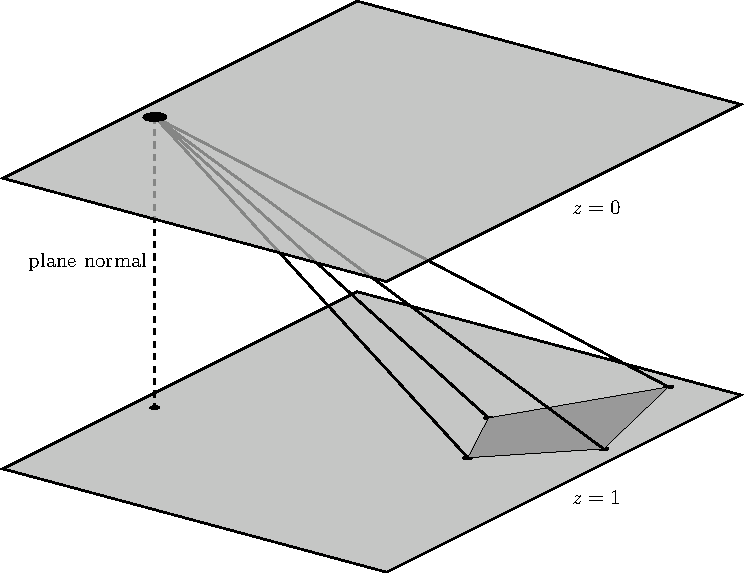
\includegraphics[width=\textwidth]{prob_geom1}
    \caption{}
    \label{fig:prob_geom:a}
\end{subfigure}
\hfill
\begin{subfigure}[b]{0.475\textwidth}
    \centering
    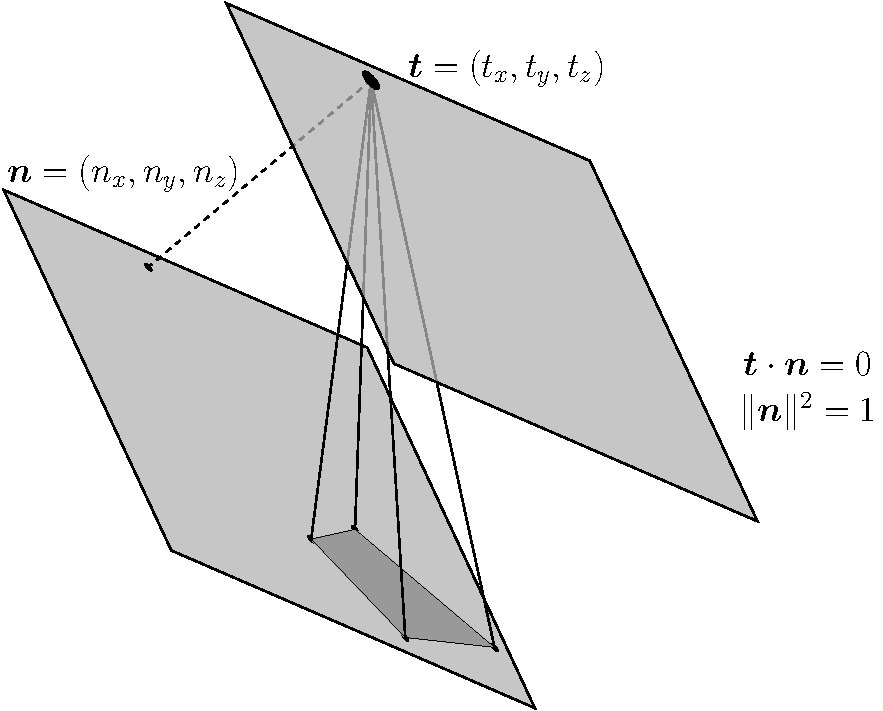
\includegraphics[width=\textwidth]{prob_geom1b}
    \caption{}
    \label{fig:prob_geom:b}
\end{subfigure}
\caption{The problem geometry considered in this paper. The camera moves in the plane $z=0$,
and is tilted about the $y$-axis an unknown angle $\theta$, followed by a rotation about
the $x$-axis by an unknown angle $\psi$, The ground floor is positioned at $z=1$.
(b)Revised problem geometry. The camera moves parallel to an unknown plane
defined by a normal vector~$\mat{n}$ of unit length.}
\label{fig:prob_geom}
\end{figure}

\emph{Solver 2}: If we re-think the geometrical interpretation, we can get a simplified system.
This was done in~\cite{valtonenoernhag-icpram-2019}:
Instead of considering the original camera matrices~\eqref{paper03:eq:cammats}, choose
the coordinate system such that
\mbox{$\mat{P}_A = [\mat{I}\,|\,\mat{0}]$},
giving $\mat{P}_B = [\mat{R}_{\mat{n}}(\phi)\,|\,-\mat{t}]$. This can be thought of
as travelling parallel to an unknown plane, as is illustrated in Figure~\ref{fig:prob_geom:a},
hence the homography can be parameterized as
\begin{equation}\label{paper03:eq:h}
    \mat{H}= \mat{R}_{\mat{n}}(\phi)+\mat{t}\mat{n}^{ \T},
\end{equation}
where $\mat{t}=(t_x,\,t_y,\,t_z)^{\T}$ is a translation vector and
\mbox{\smash {$\mat{n}=(n_x,\, n_y,\, n_z)^{\T}$}} the plane normal.
The constraint of travelling parallel
to the plane can be expressed as $\mat{t}\cdot\mat{n} = 0$ and, to fix the scale, one may
assume that~$\norm{\mat{n}}^2=1$, see~\cref{fig:prob_geom:b}.

The rotation matrix can be parameterized using quaternions. Let~$\mat{q}=(1,\,q_x,\,q_y,\,q_z)$
be a unit quaternion, then~$\mat{n}=(q_x,\,q_y,\,q_z)$
and the corresponding rotation matrix \mbox{$\mat{R}=\mat{R}(\mat{q})$}.
This results in a system in six unknowns and six equations. Furthermore, many of the multiplications
are no longer present, and is replaced with an addition; hence, the degree of the equations are
lower. We shall further compare the differences between the two solvers during the lecture.
\end{example}

\subsection{The hidden variable trick}
In certain cases, you may have a linear relationship in one or more variables in your system.
We can then use the~\emph{hidden variable trick} to eliminate these variables,
leaving a simplified system. We illustrate this in the following example from computer vision.

\begin{example}\label{ex:hidden1}
Consider the relative pose problem with known rotation and calibrated cameras.
In this case the essential matrix is $\mat{E} = [\mat{t}]_\times$. The epipolar constraint
for a pair of corresponding points $\mat{x}_i\leftrightarrow\mat{x}_i'$,
is given by $\mat{x}'^T\mat{E}\mat{x}=0$. Since the translation vector~$\mat{t}\in\R^3$,
we have two degrees of freedom (due to the scale ambiguity), and therefore we require at least
two point correspondences in order to solve the problem. The minimal problem is therefore
\begin{equation}
\begin{aligned}
    \mat{x}_1'^T\mat{E}\mat{x}_1 &= 0, \\
    \mat{x}_2'^T\mat{E}\mat{x}_2 &= 0\;.
\end{aligned}
\end{equation}
Since these equations are linear in $\mat{t}$ they can be written as
\begin{equation}
    \mat{Mt} = \mat{0},
\end{equation}
where
\begin{equation}
\mat{M} = \begin{bmatrix}
    (\mat{x}_1\times\mat{x}_1')^\T \\
    (\mat{x}_2\times\mat{x}_2')^\T
\end{bmatrix}\;.
\end{equation}
The problem is therefore reduced to finding the null space of the $2\times 3$ matrix~$\mat{M}$.
In this case it can be done explicitly using elementary operations
\begin{equation}\label{eq:2pt_optimal}
    \mat{t} = (\mat{x}_1\times\mat{x}_1') \times (\mat{x}_2\times\mat{x}_2')\;.
\end{equation}
\end{example}

It is not always the case where we get the solution directly.
You might end up with a polynomial in a single variable, in which case a
simpler root finding method can be used, \eg{} by computing the eigenvalues
of the corresponding~\emph{companion matrix}, or---if the degree of the polynomial is
less than or equal to four---a closed-form solution can be obtained. We illustrate
the latter in the following example:

\begin{example}[*]\label{ex:hidden2}
Consider the following system
\begin{equation}
\begin{aligned}
m_{11}xz + m_{12}x + m_{13}yz + m_{14}y + m_{15}z^2 + m_{16}z + m_{17} &= 0, \\
m_{22}xz + m_{22}x + m_{23}yz + m_{24}y + m_{25}z^2 + m_{26}z + m_{27} &= 0, \\
m_{32}xz + m_{32}x + m_{33}yz + m_{34}y + m_{35}z^2 + m_{36}z + m_{37} &= 0, \\
\end{aligned}
\end{equation}
where~$m_{ij}\in\C$ are generic coefficients.
By looking at a specific (non-degenerate) instance using Macaulay2
(or by using the~\emph{mixed cell method}) we see that there are in
general four solutions to this problem. One could use the action matrix method to construct an
elimination template; however, since the system is linear in $x$ and $y$ it can be rewritten as
\begin{equation}\label{eq:specialnullvector}
\mat{M}(z)
\begin{bmatrix}
x \\
y \\
1
\end{bmatrix}
= 0,
\end{equation}
where
\begin{equation}
\mat{M}(z)=
\begin{bmatrix}
    m_{11}z + m_{12} & m_{13}z + m_{14} & m_{15}z^2 + m_{16}z + m_{17} \\
    m_{22}z + m_{22} & m_{23}z + m_{24} & m_{25}z^2 + m_{26}z + m_{27} \\
    m_{32}z + m_{32} & m_{33}z + m_{34} & m_{35}z^2 + m_{36}z + m_{37}
\end{bmatrix}\;.
\end{equation}
In conclusion, we seek the one-dimensional nullspace of~$\mat{M}(z)$. Specifically, we want
the normalized null vector with the last element equal to one. This means that $\mat{M}(z)$ must
be rank deficient and therefore $\det(\mat{M}(z))=0$. Computing this gives us a
quartic polynomial in~$z$
\begin{equation}
    \det(\mat{M}(z)) =
    \alpha_4 z^4 +
    \alpha_3 z^3 +
    \alpha_2 z^2 +
    \alpha_1 z +
    \alpha_0 = 0,
\end{equation}
where $\alpha_i\in\C$ only depend on~$m_{ij}$. Specifically, we have reduced the problem to
finding the roots of a quartic polynomial which has a closed-form solution, and is fast to compute.
We do not need to resolve to other more complex methods such as the action matrix method.
When the solutions to $z$ are found, we can extract $x$ and $y$ linearly, \eg{} by using SVD
on $\mat{M}(z^*)$, for a solution $z^*$, and normalize the corresponding null vector to have
last element equal to one.
\end{example}

In the following example, which is a modification of~\cref{ex:hidden1}, we show how that
the hidden variable trick can be used to reduce the number of unknowns, but still
apply the action matrix method to the resulting system.

\begin{example}\label{ex:hidden3}
Consider the relative pose problem with known rotation but unknown and equal focal length and radial distortion.
Assume that the optical center and the distortion center coincide, and choose the local
coordinate system such that this point is at the origin. To correct for radial distortion we use
the one-parameter~\emph{division model}~\cite{fitzgibbon2001}, \ie{} the distorted
image points~$\mat{x}_d=(x,\,y,\,1)^\T$ are assumed to be mapped to their rectified counterpart~$\mat{x}_u$
using the following parametric relation
\begin{equation}
    \mat{x}_u = \phi(\mat{x}_d,\,\lambda) =
    \begin{bmatrix}
        x \\
        y \\
        1 + \lambda(x^2+y^2)
    \end{bmatrix}\;.
\end{equation}
Furthermore, the calibration matrix~$\mat{K}$ is
\begin{equation}
    \mat{K} = \begin{bmatrix}
    f\\ & f\\ && 1
    \end{bmatrix}, \qquad f > 0.
\end{equation}
In this case, the fundamental matrix is $\mat{F} = \mat{K}^{-1}[\mat{t}]_\times\mat{K}^{-1}$
and the epipolar constraint is~$\mat{x}_i'^\T\mat{Fx}_i = 0$ for two corresponding
points~$\mat{x}_i\leftrightarrow\mat{x}_i'$. Note that~$\mat{K}^{-1}$ contains $f^{-1}$ and
to make the equations polynomial we multiply each equation with~$f^2$. Furthermore, there
are four degrees of freedom (three translational parameters, the focal length and the radial
distortion coefficient, but the scale ambiguity is present); hence, the problem is minimal using four point correspondences.
More specifically, we want to solve
\begin{equation}
    f^2\cdot \phi(\mat{x}_i',\,\lambda)^\T \mat{F} \phi(\mat{x}_i,\,\lambda) = 0, \qquad \te{for }i=1,\ldots, 4.
\end{equation}
Again, the equations are linear in~$\mat{t}$ and therefore we may consider the
system
\begin{equation}
\mat{M}(f,\,\lambda)\mat{t} = 0\;.
\end{equation}
Here the matrix~$\mat{M}$ is of size $4\times 3$, and must be rank deficient to allow a non-trivial
null vector. Therefore, all $3\times 3$ minors~$\mat{M}_i$ must vanish\footnote{A
$k\times k$ \emph{minor} of a matrix~$\mat{A}$ of size $m\times n$ is the determinant of a $k\times k$ matrix obtained by removing $m-k$ rows and $n-k$ columns.}, \ie{}
\begin{equation}\label{eq:minors}
    \mat{M}_i(f,\,\lambda) = 0,  \qquad \te{for }i=1,\ldots, 4.
\end{equation}
We now have a polynomial system with four equations and two unknowns (instead of four unknowns).
\end{example}

Sometimes it is beneficial (or even necessary) to involve saturation in the process.
In practice, this is often the case when you need to enforce a special structure to the
null vector, \cf{}~\cref{ex:hidden2}. In~\cref{eq:specialnullvector} we need the last
element to be equal to one; however, this condition is lost when only enforcing the minors
to vanish.
This is also the case when considering \emph{radially-distorted conjugate translations},
which we discuss next. We will briefly outline one of the solvers from~\cite{pritts2017},
and return to it later when discussing saturation. The following text is taken verbatim from the paper:

\begin{quote}
Assume that the scene plane $\pi$ and a camera's image plane $\pi'$ are related point-wise by the
homography~$P$, so that $\alpha_i\mat{x}'_i=\mat{PX}_i$, where $\alpha_i$ is a scalar, 
$\mat{X}_i\in\pi$ and $\mat{x}'\in\pi'$. Let $\mat{X}_i$ and~$\mat{X}'_i$ be two points on the
scene plane $\pi$ such that $\mat{X}'_i -\mat{X}_i=\mat{t}$. By encoding $\mat{t}$ in the
homogeneous translation matrix $\mat{T}$, the points $\mat{X}_i$ and $\mat{X}_i$ as imaged by
camera $\mat{P}$ can be expressed as
\begin{equation}
    \alpha_i\mat{x}_i' = \mat{PX}'_i = \mat{PTX}_i = \mat{PTP}^{-1}\mat{x}_i=\mat{H_ux}_i,
\end{equation}
where the homography $\mat{H_u}=\mat{PTP}^{-1}$ is called a conjugate translation because of the
form of its matrix decomposition and points $\mat{x}_i$ and $\mat{x}'_i$ are in correspondence
with respect to the conjugate translation $\mat{H_u}$, which we denote $\mat{x}_i\leftrightarrow\mat{x}'_i$.
Decomposing $\mat{H_u}$ into its projective components gives
\begin{equation}
\alpha_i\mat{x}_i' = \left(\mat{I}_3+s_i^{\mat{u}}\mat{ul}^\T\right)\mat{x}_i
\end{equation}
where $\mat{I}_3$ is the $3\times 3$ identity matrix, and
\begin{itemize}
\item line $\mat{l}$ is the imaged scene plane’s vanishing line,
\item point $\mat{u}$ is the vanishing direction of translation, which must meet the vanishing
      line~$\mat{l}$, \ie{} $\mat{l}^\T\mat{u} = 0$,
\item and scalar $s_i^{\mat{u}}$ is the magnitude of translation in the direction $\mat{u}$ for
      the point correspondence $\mat{x}_i\leftrightarrow\mat{x}_i'$.
\end{itemize}
\end{quote}

\begin{example}\label{ex:hidden4}
Again, using the one-dimensional division model to model radial distortion, we have the
governing equations
\begin{equation}\label{eq:conjtrans}
\alpha_i \phi(\mat{x}_i',\lambda) = \left(\mat{I}_3+s_i^{\mat{u}}\mat{ul}^\T\right)\phi(\mat{x}_i,\lambda),
\end{equation}
for a pair of corresponding points~$\mat{x}_i\leftrightarrow\mat{x}_i'$ under the assumption of
conjugate translations. We will recreate the 3-point solver named H3$\mat{lu}s_{\mat{u}}\lambda$
in the paper. First, we constrain $l_3=1$ and let $\norm{\mat{u}}=s_1^{\mat{u}}$ to fix the scale
ambiguity\footnote{See the paper for more details.}.
Introduce the notation~$\bar{s}_i^{\mat{u}}\coloneqq s_i^{\mat{u}} / \norm{\mat{u}}$, which gives $\bar{s}_1^{\mat{u}}=1$. Furthermore, assume two point correspondences have the same scale of translation,
\ie{} $\bar{s}_1^{\mat{u}} = \bar{s}_2^{\mat{u}} = 1$. In this case, we have seven unknowns ($l_1$,
$l_2$, $u_1$, $u_2$, $u_3$, $\bar{s}_3^{\mat{u}}$, $\lambda$) and seven equations---two equations
per point correspondences and the orthogonality constraint~$\mat{l}^\T\mat{u}= 0$.
Since the equations are linear in~$\mat{u}$ we may write~\eqref{eq:conjtrans} as
\begin{equation}
\mat{M}(l_1,l_2,\bar{s}_3^{\mat{u}},\lambda)\begin{bmatrix} u_1 \\ u_2 \\ u_3 \\1\end{bmatrix} = 0
\end{equation}
where $\mat{M} = \mat{M}(l_1,l_2,\bar{s}_3^{\mat{u}},\lambda)$ is a $7\times 4$ matrix. It turns out that
the matrix has a special structure, namely
\begin{equation}\label{eq:pritts-M}
\mat{M} = \begin{bmatrix}
m_{11} & m_{12} &      0 & m_{14} \\
m_{21} & m_{22} &      0 & m_{24} \\
m_{31} &      0 & m_{33} & m_{34} \\
m_{41} &      0 & m_{43} & m_{44} \\
m_{51} & m_{52} &      0 & m_{54} \\
m_{61} &      0 & m_{63} & m_{64} \\
l_1 & l_2 &   1 & 0
\end{bmatrix}\;.
\end{equation}
\end{example}

As previously mentioned, by only considering the minors the structure of the null space
vector is lost.
It can happen that a one-dimensional family of false solutions is introduced corresponding
to null vectors where the last element is zero, which is the case for both~\cref{ex:hidden3}
(which is a special case of the solver proposed in~\cite{valtonenoernhag-etal-wacv-2021})
and~\cref{ex:hidden4} from~\cite{pritts2017}.
By using saturation, one may exclude such solutions, which we shall discuss later in more detail.

\subsection{Eliminating variables}
Sometimes we are able to eliminate variables even if there are no linear relationships. This
has been used by several authors~\cite{kukelova-etal-cviu-2010,fraundorfer-etal-eccv-2010,jiang-etal-accv-2014,kukelova-etal-cvpr-2015,valtonenoernhag-springer-2021}.
Consider the following toy example
\begin{example}[*]
Assume we have four unknowns $x$, $y$, $z$ and $w$, where $x^2+y^2=1$. We seek to solve
\begin{equation}
\mat{M}\mat{v} = 0,
\end{equation}
where $\mat{M}\in\C^{3\times 9}$ is a coefficient matrix and the monomial vector is
\setcounter{MaxMatrixCols}{20}
\begin{equation}
    \mat{v} = \begin{bmatrix}
            xw & x &
            yw & y &
            z^2 & zw^2 & z &
            w & 1
        \end{bmatrix}^\T\;.
\end{equation}
Due to the constraint~$x^2+y^2=1$ we cannot use the hidden variable trick. But, we can still
eliminate $z$ by using Gauss--Jordan elimination. The corresponding system, after elimination, is
on the form
\begin{equation}
\raisebox{-6pt}{ $\hat{\mat{M}} =$ }
\raisebox{-6pt}{\HUGE[}
\begingroup % keep the change local
\setlength\arraycolsep{2pt}
\begin{matrix}
%xw & x & yw & y & z^2 & zw^2 & zw & w & 1\\
z^2 & zw^2 & z & xw & x & yw & y & w & 1\\
    1 & & & \bullet & \bullet & \bullet & \bullet & \bullet & \bullet & \\
    & 1 & & \bullet & \bullet & \bullet & \bullet & \bullet & \bullet & \\
    & & 1 & \bullet & \bullet & \bullet & \bullet & \bullet & \bullet &
\end{matrix}
\endgroup
\raisebox{-6pt}{\HUGE]\;.}
\end{equation}
From the above system, we note the following relations
\begin{equation}\label{paper04:eq:elim}
    \begin{aligned}
    z^2 + g_1(x,y,w)  &=  0,\\
    zw^2 + g_2(x,y,w)  &=  0,\\
    z + g_3(x,y,w)  &=  0,\\
    \end{aligned}
\end{equation}
where~$g_i(x,y,w)$ are polynomials in the variables $x$, $y$ and~$w$.
Consequently, we must enforce the relations
\begin{equation}\label{paper04:eq:knowntilt1}
\begin{aligned}
    g_2(x,y,w) &= w^2 g_3(x,y,w), \\
    g_1(x,y,w) &= \left(g_3(x,y,w)\right)^2\;.
\end{aligned}
\end{equation}
Now, we have a reduced system with three unknowns and three equations given
by~\eqref{paper04:eq:knowntilt1} and the constraint $x^2+y^2=1$.
We will return to this problem during the lecture.

\iffalse
It turns out that~\eqref{paper04:eq:knowntilt1} are cubic and~\eqref{paper04:eq:knowntilt2} are quartic, and
by analyzing the dimension of the corresponding quotient ring, we find that
the system has six solutions in total (it can be verified that the original system has six
solutions as well). Using~\cite{larsson2018cvprb} an elimination template of size~$18\times 24$
was constructed.
\fi
\end{example}

\emph{Note:} In some cases, the elements of the coefficient matrix of the eliminated system~$\hat{\mat{M}}$ have a special structure.
This is the case in~\cite{kukelova-etal-cvpr-2015,valtonenoernhag-springer-2021}. In such cases
one must encode this structure in~$\Z_p$ when generating the elimination template.
This can, however, also happen with the hidden variable method, as in~\eqref{eq:pritts-M}.

\subsection{Saturation}
In computer vision, there are many cases where saturating a variable makes sense, \eg{}
we want the focal length to be non-zero in all practical scenarios.

\begin{example}
Consider~\cref{ex:hidden3}. The system~\eqref{eq:minors} has infinitely many solutions; however,
many of these correspond to solutions where~$f=0$. If we saturate~$f$ there are finitely many solutions.
\end{example}

The automatic generator supports saturating an ideal w.r.t.\@ a monomial. In many situations, one might
want to remove more complex degeneracies, \eg{} one might want to enforce a homography~$\mat{H}$
to be invertible, hence~$\det{\mat{H}}\neq 0$. If you want to saturate a polynomial~$f$ this
can still be accomplished by introducing a new
variable~$x_0$ as well as the constraint~$x_0-f(\mat{x}) = 0$.
Another way of eliminating certain solutions is by using the \emph{Rabinowitsch trick}\footnote{This
is often used when proving Hilbert's Nullstellensatz (\cf{} Theorem 2, p. 173, in~\cite{cox}) from the weak
Nullstellensatz.},
which is to introduce~$x_0f(\mat{x})-1 = 0$.
We show in an example that using saturation produces smaller elimination
templates.\footnote{Empirically, this is often true. One argument for why this is the case
is because the auxiliary variable $x_0$ is linear in the equation and therefore easier to eliminate.}
Furthermore, one may exclude the auxiliary variable~$x_0$ from the quotient ring basis
(when saturating polynomials).

\begin{example}[*]
We return to~\cref{ex:hidden4} and show how to remove the one-dimensional family of solutions
corresponding to null vectors with the last element equal to zero.
First, since~$\mat{M}$ in~\eqref{eq:pritts-M} is of size~$7\times 4$ there are $\binom{7}{4}=35$
different minors; hence, we have reduced the system to 35 equations in four unknowns.
If one would try to find a Gröbner basis to such an instance, however, Macaulay2 would
cast an error saying:~\texttt{module given is not finite over the base}. This is because
there is a one-dimensional family of null vectors with last element equal to zero. To remove
these we may saturate any of the $3\times 3$ minors from the first three columns of~$\mat{M}$.
Following the suggestions by the authors, we choose the one with the lowest degree, corresponding
to the two first rows and the last row
\begin{equation}
    f_s =
        \begin{vmatrix}
        m_{11} & m_{12} & 0\\
        m_{21} & m_{22} & 0\\
        l_1 & l_2 &   1
        \end{vmatrix}
        =
        m_{11}m_{22}-m_{12}m_{21}\;.
\end{equation}
We add an auxiliary variable $x_{\te{aux}}$ and  the equation~$x_{\te{aux}}-f_s(l_1,l_2,\bar{s}_3^{\mat{u}},\lambda) = 0$. This gives us 36 equations in five unknowns. We will return to this example
during the lecture.

It turns out that the elimination template is of size~$22\times 24$.\footnote{Note that it is not
the same as in the paper---we are using a slightly different approach. But, potentially, we have
a better solver as the state-of-the-art solver in~\cite{pritts2017} is of size~$24\times 26$.}
This assumes that we use a basis without the auxiliary variable. Using the Rabinowitsch trick,
we instead get an elimination template of size $59\times 61$.
\end{example}

\subsection{Using symmetries}
This is based on~\cite{larsson2016eccv}; however, we will not discuss it during the lecture,
to limit the scope slightly; however, I feel that the document would be incomplete without
mentioning it. Hence, there are a few example code snippets available for you to try on your own.

\begin{example}[*]
Twofold symmetries using quaternion parameterization (see Section~3.4 in~\cite{larsson-phd}).
\end{example}

\pexamples~\cite{larsson-etal-cvpr-2018,wu-cvpr-2015}.

\subsection{A clever elimination strategy}
This section is based on~\cite{kukelova-etal-2017-cvpr}. We reproduce some of the material
here verbatim:

\begin{quote}
In computer vision, we often encounter polynomial systems in which only the linear equations~$F_L$
depend on image measurements, while the nonlinear equations~$F_N$ stay the same, regardless of
image measurements. For example, the epipolar constraint generates linear equations that depend
on the input measurements while the singularity of the fundamental matrix results in the non-linear
equation~$\det(F) = 0$, which does not depend on the measurements. Here we present a new ``clever''
elimination strategy, which usually allows us to do more computation in the off-line stage and less
computation in the online stage.
Throughout this section we assume that the nonlinear equations~$F_N$ do not depend on image
measurements, \ie{} for all instances these equations are the same.
[\ldots]
Let us now describe our new elimination strategy. We first divide the input equations~$F$ into the
linear equations~$F_L$ and the non-linear equations~$F_N$. Moreover, we divide the $n$ given unknowns
$X$ into two subsets:
\begin{equation}
    \begin{aligned}
        X_L &= \{x_i\in X\;|\;x_i\text{ appears in some }f\in F_L\}\\
        X_N &= X\setminus X_L.
    \end{aligned}
\end{equation}
The set $X_L$ contains the unknowns that appear in linear equations. The set $X_N$ contains the
unknowns that appear in equations of higher degree only. We fix the following notation:
$|F_L|=m_L$, $|F_N|=mN$, $|X_L|=n_L$, $|X_N|=n_N$, which means that $m=m_L+m_N$ and $n=n_L+n_N$.
In more detail, our method performs the following steps.
\pagebreak
\paragraph{Offline:}
\begin{enumerate}
    \item Let $I = \langle F_N \rangle$ and consider the elimination
    ideal~$I_{X_L}=I\cap \C[X_L]$
    \item Compute the generators $G$ of $I_{X_L}$. These contain unknowns from $X_L$ only, \ie{}
    the unknowns appearing in the linear equations $F_L$.
\end{enumerate}
\paragraph{Online:}
\begin{enumerate}[resume]
    \item Rewrite the linear equations $F_L$ in the unknowns $X_L$ as $\mat{M}X_L= 0$, where $\mat{M}$
    is a coefficient matrix and the vector $X_L$ contains all unknowns from $X_L$.
    \item Compute a null space basis $\mat{N}$ of $\mat{M}$ and re-parametrize the unknowns $X_L=\mat{N}Y$. If the
    rank of $\mat{M}$ is $m_L$, \ie{} the equations in $F_L$ are linearly independent, $Y$ would contain
    $k=n_L - m_L$ new unknowns. Note that if all input equations in $F$ were homogeneous, we could
    set one of the unknowns in $Y$ to 1 (assuming it is non-zero) and then $k=n_L-m_L-1$.
    \item Substitute $X_L=NY$ into the generators $G$ of the elimination ideal $I_{X_L}$.
    \item Solve the new system of polynomial equations $G(Y) = 0$ (\eg{} using the Gröbner basis
    method and the precomputed elimination template for~\mbox{$G(Y) = 0$} obtained by using the automatic
    generator \cite{kukelova2008}).
    \item Back-substitute to recover $X_L=\mat{N}Y$.
    \item Extend partial solutions for $X_L$ to solutions for $X$.
\end{enumerate}
The main difference between our elimination strategy and the elimination strategies used before in
minimal solvers (see Section2.1.2) is that the previous strategies substitute the parametrization
$X_L=NY$ directly into the input nonlinear equations $F_N$. This results in $m_N$ polynomial
equations in $n_N+k$ unknowns $Y\cup X_N$. On the other hand, the new method eliminates
$n_N$ unknowns from the non-linear equations and creates a system $G(Y) = 0$ in $k$ unknowns in the
pre-processing step. We will show on several important problems from computer vision that solving
the system $G(Y)  =  0$, instead of the system $F_N(Y\cup X_N) = 0$, is more efficient.
\end{quote}

Here is an example of how this strategy can be used.
\begin{example}[*]
Let us continue from~\cref{ex:Hplanar1}.
Following the suggested approach proposed by Kukelova~\etal{} we
consider the ideal generated by
\mbox{$\lambda \mat{H}-\mat{R}(\mat{q})-\mat{tn}^{T}=0$}, where $\lambda$ is a scale factor,
and $\mat{t}\cdot\mat{n}=0$. Let it be denoted~$I$,
then we seek the elimination ideal~$I\cap\K[\mat{H}]$, for some suitable field~$\K$.
Over a finite field, this can be done using Macaulay2. We will do this during the lecture, which
concludes the offline stage of the proposed elimination strategy.
This results in the eleven quartic constraints originally found
in~\cite{wadenback2016}\footnote{
These constraints were experimentally obtained by randomly generating points on the manifold defining
the planar motion compatible homographies.
In order to be able to work over a finite field, the rotation matrices were constructed
using Pythagorean triplets, hence integer versions of the problem were obtained. By doing so,
the coefficients for the polynomials could be found.
With this approach, however, one cannot rule out the existence of higher-order polynomials,
and thus, sufficiency cannot be proven.} and an additional sixth degree polynomial.

Now, we parameterize the null space of the homography using 2.5-point correspondences, \ie{}
given three corresponding points $\mat{x}_i \leftrightarrow \mat{x}'_i$ for $i=1,2,3$, we get
\begin{equation}
    \mat{x}_i'\times \mat{Hx}_i = 0,
\end{equation}
and choosing two linearly independent rows (apart from the third pair, where we only pick one row),
from which we get a system
\begin{equation}
\mat{M}\mat{H} = 0,
\end{equation}
where $\mat{M}$ is a $5\times 9$ matrix. Assuming non-degenerate configurations, the matrix $\mat{M}$
has a four-dimensional null space ant we may write it in terms of the basis elements
\begin{equation}
    \mat{H} = \sum_{i=1}^4\lambda_i\mat{H}_i\;.
\end{equation}
Note that there is a scale ambiguity, therefore we may lock the scale \eg{} by forcing \mbox{$\lambda_4=1$}.
Now, this corresponds to steps 3 and 4 of the online stage of the elimination strategy proposed by
Kukelova~\etal{}. We now use this parameterization of the three unknowns~$\lambda_i$, for $i=1,2,3$
and insert them in the generators (the eleven quartic equations). This yields a new system
\begin{equation}
\begin{aligned}
    g_1(\lambda_1,\lambda_2,\lambda_3) &= 0, \\
    &\vdots \\
    g_{11}(\lambda_1,\lambda_2,\lambda_3) &= 0,
\end{aligned}
\end{equation}
for which the action matrix method is applicable. We will return to this example during the lecture.
\end{example}

\begin{example}
Study the example of relative pose with unknown focal length,
from~\cite{kukelova-etal-2017-cvpr}.
\end{example}

\pexamples~\cite{kukelova-etal-2017-cvpr,ding-etal-2019-iccv,barath-kukelova-iccv-2019,valtonenoernhag-icpram-2019}

\subsection{Beyond Gröbner bases}
This section is based on~\cite{larsson2018cvpr} and utilizes the fact that one does not
have to use a Gröbner basis in order to generate the elimination template.
This can lead to smaller elimination template sizes.

\pexamples~\cite{valtonenoernhag-springer-2021}

\subsection{Using PEP and other approaches for numerical stability and/or speed}
See also~Section 1.3.3 in~\cite{larsson-phd}.
Ding~\etal{} transformed their problem to a \emph{polynomial eigenvalue problem} (PEP)
to increase both numerical accuracy and speed \cite{ding-etal-tpami-2020,ding-etal-cvpr-2020}.
Furthermore, they prove a result similar to saturation in this setting---namely how to remove
zero (generalized) eigenvalues by row and column operations prior to solving the PEP. This makes the dimension
of the coefficient matrices of the PEP smaller, which benefits the overall performance.

\subsection{The latest on resultant based methods}
In \cite{bhayani-etal-cvpr-2020,bhayani-etal-arxiv-2020} automatic generators using
resultant-based methods are proposed. Major strengths compared to the action matrix method is
in terms of numerical stability.

\subsection{What about large scale problems?}
Gröbner basis methods only work well when the number of solutions are small---say less than one
hundred solutions---since larger solvers suffer from numerical instability, due to large eliminations
and eigenvalue problems. One way to approach larger problems is by using \emph{homotopy continuation} (HC). In computer vision, a famous problem with many solutions is the trifocal problem, \ie{} with
three calibrated cameras. There are two common minimal problems for points and lines in three views
with 216 and 312 solutions each. These are considerd in~\cite{fabbri-etal-cvpr-2020}, and they also
propose the C++ package called MINUS (MInimal problem NUmerical Solver), which is publicly available.\footnote{Code available at~\url{https://github.com/rfabbri/minus}.}

\clearpage
\bibliographystyle{apalike}
{\small
\bibliography{alggeom_lecture_marcus}}

\end{document}
